\documentclass{../../text-style}

\texttitle{Лекция 10: Сопровождение и реинжиниринг}

\begin{document}

\maketitle
\thispagestyle{empty}

\attribution{Тимофей Александрович Брыксин, бывш. доцент кафедры системного программирования СПбГУ}

Невозможно создать систему, которая не потребует изменений в будущем. Как только программное обеспечение вводится в эксплуатацию, из-за постоянного развития бизнес-процессов компании и окружающей её среды возникают новые требования к системе. Иногда в системе следует изменить некоторые составляющие в целях повышения производительности или улучшения других характеристик, а также для исправления обнаруженных ошибок. Все это требует дальнейшего развития системы после ее ввода в эксплуатацию. При этом организации часто попадают в зависимость от используемого программного обеспечения, так что приходится дополнительно вкладываться в его эволюцию, чтобы поддерживать уровень его производительности.

\section{Динамика развития программ}

Под динамикой развития программ подразумевается исследование изменений в программной системе. Результатом этих исследований стало появление ряда <<законов>> Лемана\footnote{Про них в Википедии: \url{https://ru.wikipedia.org/wiki/Законы_Лемана} (дата обращения: 29.04.2023).}, относящихся к модернизации систем. Они сформулированы в период с 1974 по 1996 годы после исследования процесса создания и эволюции ряда больших программных систем. Приведём их в том виде, в котором они были сформулированы, и проанализируем.

\begin{itemize}
    \item \textbf{Непрерывное изменение}: используемая система должна непрерывно адаптироваться под изменяющийся мир, иначе её полезность снижается.
    \item \textbf{Увеличение сложности}: по мере того, как программа эволюционирует, её сложность растёт, если не производится работ по стабилизации и уменьшению сложности.
    \item \textbf{Саморегулирование}: процесс эволюции программы является саморегулируемым, с близким к нормальному распределению масштабом атрибутов продукта и процесса.
    \item \textbf{Сохранение организационной стабильности} (неизменная скорость работы): средний эффективный глобальный уровень активности в эволюционирующей системе инвариантен к времени жизни продукта.
    \item \textbf{Сохранение осведомлённости}: в течение активной жизни эволюционирующей программы основное содержание последующих релизов статистически неизменно.
    \item \textbf{Ухудшение качества}: качество программ будет восприниматься как ухудшающееся, если они не сопровождаются должным образом и не адаптируются к операционной среде.
    \item \textbf{Система обратной связи}: процессы программирования вместе составляют многоконтурные, многоуровневые системы обратной связи и должны рассматриваться как таковые, чтобы успешно изменяться и улучшаться.
\end{itemize}

Из первого закона вытекает необходимость постоянного сопровождения системы. При изменении окружения, в котором работает система, появляются новые требования, и система должна неизбежно изменяться, чтобы им соответствовать. Изменения системы носят циклический характер, когда новые требования порождают появление новой версии системы, что, в свою очередь, вызывает изменения системного окружения; это находит отражение в формировании новых требований к системе и т.д.

Второй закон констатирует нарушение структуры системы после каждой модификации. Это в полной мере демонстрируют унаследованные (legacy) системы, которые будем обсуждать чуть далее. Единственным способом избежать этого, по всей видимости, является только профилактическое обслуживание, которое, однако, требует средств и времени. При этом совершенствуется структура программы без изменения ее функциональности. Поэтому в бюджете, предусмотренном на содержание системы, следует также учесть и эти дополнительные затраты.

Самым спорным и, пожалуй, самым интересным законом Лемана является третий. Согласно этому закону, все большие системы имеют собственную динамику изменений, которая устанавливается на начальном этапе разработки системы. Этим определяются возможности сопровождения системы и ограничивается количество модификаций. Предполагается, что этот закон является результатом действия фундаментальных структурных и организационных факторов. Как только система превышает определенный размер, она начинает действовать подобно некой инерционной массе. Размер становится препятствием для новых изменений, поскольку эти изменения с большой вероятностью станут причиной ошибок в системе, которые снизят эффективность нововведений в новой версии системы.

Четвертый закон Лемана утверждает, что крупные проекты по разработке программного обеспечения действуют в режиме <<насыщения>>. Это означает, что изменения ресурсов или персонала оказывает незначительное влияние на долгосрочное развитие системы. Это, правда, уже указано в третьем законе, который утверждает, что развитие программы не зависит от решений менеджмента. Этим законом также утверждается, что крупные команды программистов неэффективны, так как время, потраченное на общение и внутрикомандные связи, превышает время непосредственной работы над системой.

Пятый закон затрагивает проблему увеличения количества изменений с каждой новой версией программы. Расширение функциональных возможностей системы каждый раз сопровождается новыми ошибками в системе. Таким образом, масштабное расширение функциональных возможностей в одной версии означает необходимость последующих доработок и исправления ошибок. Поэтому в следующей версии уже будут проведены незначительные модификации. Таким образом, менеджер, формируя бюджет для внесения крупных изменений в версию системы, не должен забывать о необходимости разработки следующей версии с исправленными ошибками предыдущей версии.

\section{Унаследованные (legacy) системы}

Для разработки программного обеспечения компании обычно должны заплатить немалую сумму. Естественно, чтобы оправдать эти затраты, программные продукты должны находиться в использовании и приносить пользу по крайней мере несколько лет. Жизненный цикл программ может быть самым разным, но, как правило, большие системы успешно функционируют и более десяти лет. Некоторые компании не отказываются и от таких систем, которым уже по 20 лет и более\footnote{См., например, \url{https://blog.codinghorror.com/cobol-everywhere-and-nowhere/} (дата обращения: 29.04.2023).}. От многих из них все еще зависит деятельность этих компаний, и малейшая ошибка в системе приводит к сбою их деловой активности. Именно такие системы и получили название наследуемых или унаследованных (legacy systems).

Эволюция экономики, изменения рынка, законов, менеджмента, структурные преобразования в компании и т.п. служат причиной появления новых или изменения существующих требований к программному обеспечению, что непосредственно приводит к модификации существующих систем. За несколько лет наследуемая система может пережить целый ряд подобных изменений, совершаемых разными специалистами, поскольку одному человеку практически невозможно полностью освоить систему во всех аспектах.

Бизнес, как правило, настроен на систематическое обновление и модернизацию существующего аппаратного обеспечения. Однако, что касается списания и замены наследуемых систем современным программным обеспечением, такие действия могут повлечь за собой серьезный риск и необратимые последствия в деятельности компаний. Ввиду этого многие менеджеры не желают рисковать, устанавливая неизвестное и непредсказуемое современное программное обеспечение, и продолжают использовать старые системы. Замена наследуемой системы~--- дело рискованное по многим причинам.

\begin{itemize}
    \item Редко можно найти такую наследуемую систему, которая имеет полное и точное техническое описание. Старое описание может быть утеряно, а если оно и существует, вряд ли там будут указаны все изменения, сделанные в системе за годы её жизни. Поэтому трудно сравнивать технические характеристики и функциональные возможности старой системы с характеристиками ее возможной замены.
    \item Функционирование унаследованной системы тесно связано с деловой активностью компании. При замене системы деятельность компании также претерпит изменения, что может привести к непредсказуемым расходам и необратимым последствиям.
    \item Некоторые встроенные в систему правила, регулирующие область деятельности компании, могут быть нигде не документированы. Эти правила обеспечивают своеобразные рамки, в которых должна вестись коммерческая деятельность, и нарушение этих рамок окажет не самое лучшее влияние на развитие бизнеса. 
    \item Создание новых программных систем связано с риском, так как новизна системы подразумевает появление непредусмотренных проблем. Разработчик программного обеспечения может поставить программный продукт не вовремя, либо может измениться цена его разработки.
\end{itemize}

Использование наследуемых систем избавляет организацию от риска, связанного с их заменой. Однако модернизация старой системы становится дороже с каждым годом эксплуатации. Возрастающая стоимость модернизации системы, находящейся в эксплуатации несколько лет, определяется следующими факторами.

\begin{itemize}
    \item Отдельные части системы разрабатывались разными командами программистов, поэтому в них отсутствует единство стиля программирования.
    \item Система либо ее отдельные части могут быть написаны с помощью языков, давно вышедших из употребления. Трудность подбора специалистов, знающих эти языки и технологии, усугубляется дорогостоящими договорами на внешнее сопровождение системы.
    \item Документация системы часто бывает устаревшей и не отвечает современным требованиям. Иногда единственной документацией может остаться исходный код программ. В особо трудных случаях исходный код давно утерян, и все, что доступно,~--- это функционирующая версия программы.
    \item Долгие годы эксплуатации могут оказать разрушительное воздействие на архитектуру системы и исказить ее настолько, что она станет практически недоступной для понимания. Кроме того, в систему могут быть добавлены либо подогнаны к ней другие программы.
    \item Система может быть оптимизирована для экономного использования памяти или для быстрого выполнения. Это создает дополнительные трудности для программистов, владеющих современными технологиями инженерии программного обеспечения, но не имеющих понятия о хитростях и тонкостях программирования данной системы.
    \item Данные, с которыми работает система, могут содержаться в разных источниках с несовместимыми структурами. Отсюда высокая вероятность дублирования данных, кроме того, они могут быть устаревшими, неполными либо неточными.
\end{itemize}

Организация, использующая большое количество наследуемых систем, сталкивается с серьезной проблемой. Продолжая использовать и модернизировать наследуемые системы, она тем самым значительно повышает свои расходы.

\subsection{Оценивание наследуемых систем}

Организации, деятельность которых во многом зависит от наследуемых систем, и средства которых на их сопровождение и модернизацию ограничены, должны хорошо подумать над тем, как получить максимум от вложений в наследуемую систему. Это прежде всего означает корректную оценку наследуемой системы и выбор наиболее подходящей стратегии ее модернизации. Существует несколько стратегических путей решения этой задачи.

\begin{center}
    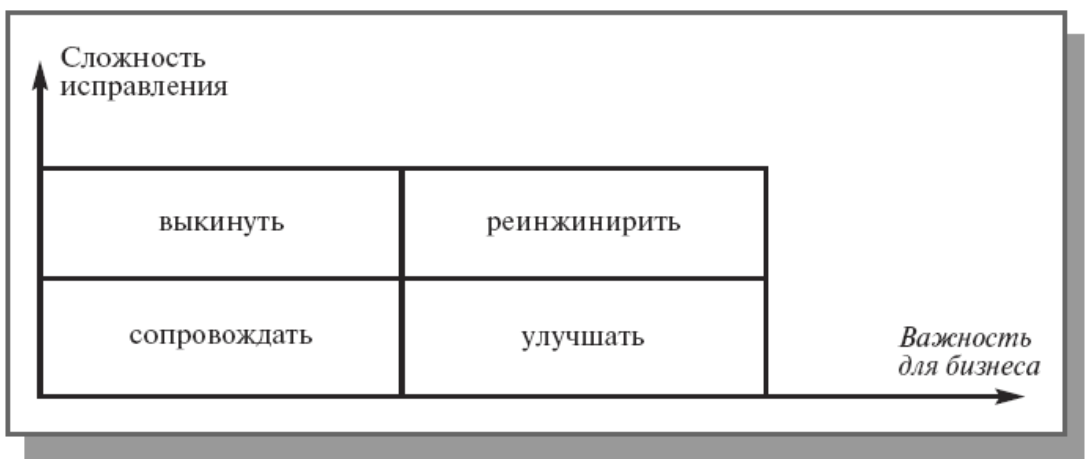
\includegraphics[width=0.7\textwidth]{maintenanceWays.png}
\end{center}

\begin{itemize}
    \item \textbf{Полностью отказаться от системы}. Это решение применимо в случае, если система не отвечает своим задачам поддержки бизнес-процессов. Например, со времени установки системы бизнес-процессы изменились настолько, что уже практически не зависят от работы системы. Чаще всего это случается там, где универсальные ЭВМ были заменены персональными компьютерами, а устаревшее программное обеспечение было модернизировано в той мере, в которой это необходимо для продолжения его работы на ПК.
    \item \textbf{Продолжить сопровождение системы}. Это решение подходит в ситуациях, когда система более или менее стабильна и всё ещё полезна в работе, а пользователи не требуют ее значительного изменения.
    \item \textbf{Модернизировать систему для улучшения сопровождения}. Этот путь следует выбрать тогда, когда качество работы системы снизилось в результате частых изменений, причем дальнейшие изменения все ещё нужны, но при этом их внесение не особо проблемно.
    \item \textbf{Заменить старую систему более новой}. Этот вариант применяется в том случае, если в связи с появлением современных аппаратных средств старая система становится непригодной к эксплуатации, но при этом её важность для компании велика. Это может быть покупка аналогичной системы, реинжиниринг старой или создание новой системы с нуля.
\end{itemize}

Естественно, нет однозначного решения данной проблемы~--- к системе, состоящей из нескольких отдельных программ, можно применить несколько различных подходов.

При оценивании наследуемую систему нужно рассматривать под разными углами зрения. С коммерческой точки зрения необходимо провести оценку полезности и пригодности системы для бизнеса. Что же касается перспективы дальнейшей работы системы, нужно в первую очередь оценить качество прикладного программного обеспечения, а также программных и аппаратных средств поддержки данной системы. Комбинация двух оценок~--- бизнес-пригодность и качество~--- поможет решить, что же делать с наследуемой системой дальше.

\section{Модернизация программного обеспечения}

Приведенные выше стратегии по модернизации программных систем не исключают одна другую. Например, иногда для упрощения системы перед изменением архитектуры или для переделки некоторых ее компонентов применяется реинжиниринг.

Разные стратегии могут также применяться к отдельным частям системы или к отдельным программам наследуемой системы. Сопровождение приемлемо для программ со стабильной и четкой структурой, не требующей особого внимания. Для других программ, которые постоянно контактируют со многими пользователями, можно изменить архитектуру так, чтобы интерфейс пользователя запускался на машине клиента. Еще один компонент в этой же системе можно заменить аналогичной программой стороннего производителя. Однако при реинжиниринге обычно необходимо изменять все компоненты системы.

\subsection{Сопровождение}

Сопровождение~--- это обычный процесс изменения системы после ее поставки заказчику. Эти изменения могут быть как элементарно простыми (исправление ошибок программирования), так и более серьезными, связанными с корректировкой отдельных недоработок либо приведением в соответствие с новыми требованиями. Сопровождение не связано со значительным изменением архитектуры системы. При сопровождении тактика простая: изменение существующих компонентов системы либо добавление новых.

Существует четыре вида сопровождения системы.

\begin{itemize}
    \item \textbf{Сопровождение с целью исправления ошибок.} Обычно ошибки в программировании достаточно легко устранимы, однако ошибки проектирования стоят дорого и требуют корректировки или перепрограммирования некоторых компонентов. Самые дорогие исправления связаны с ошибками в системных требованиях, так как здесь может понадобиться перепроектирование системы.
    \item \textbf{Сопровождение с целью адаптации программного обеспечения к специфическим условиям эксплуатации.} Это может потребоваться при изменении определённых составляющих рабочего окружения системы, например аппаратных средств, операционной системы или программных средств поддержки. Чтобы адаптироваться к этим изменениям, система должна быть подвергнута определенным модификациям.
    \item \textbf{Сопровождение с целью изменения функциональных возможностей системы.} В ответ на организационные или деловые изменения в организации могут измениться требования к программным средствам. По статистике это наиболее часто применяемый вариант сопровождения.
    \item \textbf{Профилактическое сопровождение.} Модификация программного продукта на этапе эксплуатации для повышения удобства сопровождения, а также идентификации и предотвращения скрытых дефектов до того, когда они приведут к реальным сбоям.
\end{itemize}

На практике однозначно четкое разграничение между различными видами сопровождения провести достаточно сложно. Ошибки в системе могут быть выявлены в том случае, если, например, система использовалась непредсказуемым способом. Поэтому наилучший способ исправления ошибок~--- расширение функциональных возможностей программы с тем, чтобы сделать работу с ней как можно проще. При адаптации программного обеспечения к новому рабочему окружению расширение функциональных возможностей системы будет способствовать улучшению ее работы. Также добавление определенных функций в программу может оказаться полезным, если в случае ошибок был изменен шаблон использования системы и побочным действием при расширении функциональных возможностей будет удаление ошибок.

Найти современные данные относительно того, как часто используется тот или иной тип сопровождения, довольно сложно. Согласно исследованиям\footnote{\url{https://dl.acm.org/doi/book/10.5555/601062} )(дата обращения: 30.04.2023).}, которые были проведены в 1980 году, 65\% сопровождения связано с выполнением новых требований, 18\% отводится на изменения системы с целью адаптации к новому окружению и 17\% связано с исправлением ошибок. Десятилетие спустя в другой работе\footnote{\url{https://dl.acm.org/doi/10.1002/smr.4360020303} )(дата обращения: 30.04.2023).} были определены похожие соотношения. Из этого можно определить, что исправление ошибок не является самым распространенным видом сопровождения. Модернизация системы в соответствии с новым рабочим окружением либо в соответствии с новыми требованиями более эффективна. Поэтому сопровождение само по себе является естественным процессом продолжения разработки системы со своими процессами проектирования, реализации и тестирования. Таким образом, инкрементально-итеративные модели разработки вполне могут продолжать использоваться и на этапе сопровождения.

Соотношение между величинами средств на сопровождение и на разработку может быть разным в зависимости от предметной области, где эксплуатируется система. Для прикладных систем, работающих в деловой сфере, соотношение затрат на сопровождение в основном сравнимо со средствами, потраченными на разработку. Для встроенных систем реального времени затраты на сопровождение могут в несколько раз превышать стоимость самой разработки. Высокие требования в отношении производительности и надежности таких систем предполагают их жесткую структуру, которая труднее поддается модификации.

Причиной высоких затрат на сопровождение является сложность модернизации системы после ее внедрения, поскольку расширить функциональные возможности намного легче в процессе создания системы. Ниже приведены ключевые факторы, которые определяют стоимость разработки и сопровождения и могут привести к подорожанию сопровождения.

\begin{itemize}
    \item \textbf{Стабильность команды разработчиков}. Как часто бывает, после внедрения системы команда разработчиков распадается, эти специалисты будут работать над другими проектами. Новым членам команды или же отдельным специалистам, которые возьмут на себя дальнейшее сопровождение системы, будет трудно понять все ее особенности. Поэтому на понимание системы перед внесением в неё изменений уходит много времени и средств.
    \item \textbf{Ответственность согласно контракту}. Контракт на сопровождение обычно заключается отдельно от договора на разработку программы. Более того, иногда контракт на сопровождение может получить фирма, сама не занимающаяся разработкой. Вместе с фактором нестабильности команды это может стать причиной отсутствия в команде стимула создать легкоизменяемую, удобную в сопровождении систему. Если членам команды выгодно пойти кратчайшим путем с минимальными затратами усилий, то вряд ли они откажутся от этого даже с риском повышения последующих затрат на сопровождение.
    \item \textbf{Квалификация специалистов}. Специалисты, занимающиеся сопровождением, часто не знакомы с предметной областью, где эксплуатируется система. Сопровождение не пользуется популярностью среди разработчиков. Это считается менее квалифицированной разработкой и часто поручается младшему персоналу. Более того, старые системы могут быть написаны на устаревших языках программирования, не знакомых молодым специалистам и требующих дополнительного изучения.
    \item \textbf{Возраст и структура программы}. С возрастом структура программ нарушается вследствие частых изменений, поэтому их становится сложнее понимать и изменять. Кроме того, многие наследуемые системы были созданы без использования современных технологий. Они никогда не отличались хорошей качественной структурой; изменения, сделанные в них, были направлены скорее на повышение эффективности функционирования, чем на повышение удобства сопровождения. Документация на старые системы часто бывает неполной либо вообще отсутствует.
\end{itemize}

Первые три проблемы объясняются тем, что многие организации все еще делают различие между разработкой системы и ее сопровождением. Сопровождение считается делом второстепенным, поэтому нет никакого желания инвестировать средства для снижения затрат на будущее сопровождение. И руководству организаций, и разработчикам полезно помнить, что у систем редко бывает четко определенный срок функционирования, наоборот, они могут находиться в эксплуатации в той либо иной форме неограниченное время.

Дилемма заключается в следующем: или создавать системы и поддерживать их до тех пор, пока это возможно, и затем заменять их новыми, или разрабатывать постоянно эволюционирующие системы, которые могут изменяться в соответствии с новыми требованиями. Их можно создавать на основе наследуемых систем, улучшая структуру последних с помощью реинжиниринга, либо путем изменения архитектуры этих систем.

Последняя проблема, а именно нарушение структуры, является самой простой из них. Технология реинжиниринга поможет усовершенствовать структуру и повысить понимаемость системы. В подходящих случаях адаптировать систему к новым аппаратным средствам может и модернизация архитектуры. Профилактические меры при сопровождении будут полезны, если возникнет необходимость усовершенствовать систему и сделать ее более удобной для изменений.

\subsubsection{Процесс сопровождения}

Процессы сопровождения могут быть самыми разными, что зависит от типа программного обеспечения, технологии его разработки, а также от специалистов, которые непосредственно занимались созданием системы. Во многих организациях сопровождение носит неформальный характер, в большинстве случаев разработчики получают информацию о проблемах системы от самих пользователей в устной форме. Другие же компании имеют формальный процесс сопровождения со структурированной документацией на каждый его этап. Но на самом общем уровне любые процессы сопровождения имеют общие этапы, а именно: анализ изменений, планирование версий, реализация новой версии системы и поставка системы заказчику.

\begin{center}
    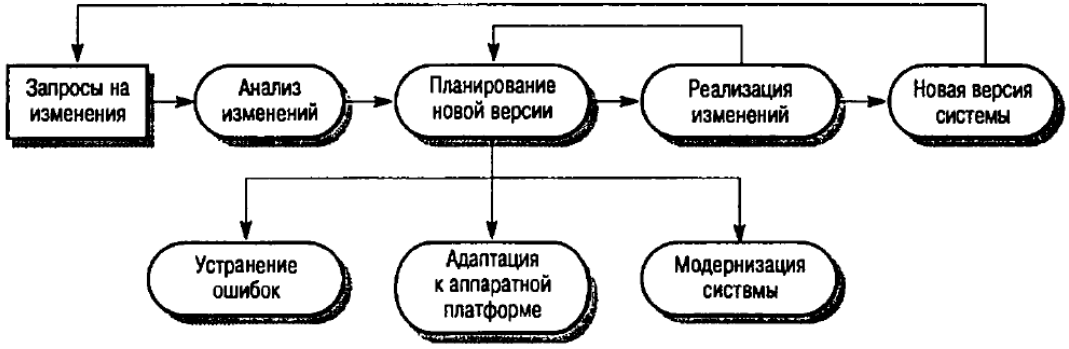
\includegraphics[width=0.95\textwidth]{maintenanceProcess.png}
\end{center}

Процесс сопровождения начинается при наличии достаточного количества запросов на изменения от пользователей, менеджеров или покупателей. Далее оцениваются возможные изменения с тем, чтобы определить уровень модернизации системы, а также стоимость внедрения этих изменений. Если принимается решение о модернизации системы, начинается этап планирования новой версии системы. Во время планирования анализируется возможность реализации всех необходимых изменений, будь то исправление ошибок, адаптация или расширение функциональных возможностей системы. Только после этого принимается окончательное решение о том, какие именно изменения будут внесены в систему.

Но в экстренных случаях требуется быстрое внесение изменений, например по следующим причинам:

\begin{itemize}
    \item сбой в системе, вследствие чего возникла чрезвычайная ситуация, требующая экстренного вмешательства для продолжения нормальной работы системы;
    \item изменение рабочего окружения системы с непредусмотренным влиянием на систему;
    \item неожиданные изменения в деловой сфере организации (из-за действий конкурентов или из-за введения нового законодательства).
\end{itemize}

В таких случаях быстрая реализация изменений имеет большую важность, чем четкое следование формальностям процесса модернизации системы. Вместо того чтобы изменять требования или структуру системы, возникает необходимость быстро внести коррективы в программный код. Однако этот подход опасен тем, что требования, системная архитектура и программный код постепенно теряют целостность. Этого трудно избежать, если принять во внимание необходимость быстрого выполнения задания, когда тщательная доработка системы откладывается на потом. Если разработчик, который изменил код, внезапно уходит из команды, то его коллеге будет сложно привести в соответствие сделанным изменениям спецификацию и структуру системы.

Еще одна проблема срочных изменений системы состоит в том, что из-за дефицита времени из двух возможных решений будет принято не самое лучшее (в аспекте сохранения структуры системы), а то, которое можно быстрее и эффективнее реализовать. В идеале после срочной коррекции кода системы запрос на изменения должен все еще оставаться в силе. Поэтому после тщательного анализа изменений можно отменить внесенные изменения и принять более оптимальное решение для модернизации системы. Однако на практике такая возможность используется крайне редко, чаще всего в силу нехватки времени и наличия других <<горящих>> задач.

\subsubsection{Прогнозирование сопровождения}

Менеджеры терпеть не могут сюрпризов, особенно если они выливаются в непредсказуемо высокие затраты. Поэтому лучше предусмотреть заранее, какие изменения возможны в системе, с какими компонентами системы будет больше всего проблем при сопровождении, а также рассчитать общие затраты на сопровождение в течение определенного периода времени. 

Прогнозирование количества запросов на изменения системы зависит от понимания взаимосвязей между системой и ее окружением. Некоторые системы находятся в достаточно сложной взаимозависимости с внешним окружением и изменение окружения обязательно повлияет на систему. Для того чтобы правильно судить об этих взаимоотношениях, необходимо оценить следующие показатели.

\begin{itemize}
    \item \textbf{Количество и сложность интерфейсов}. Чем больше системных интерфейсов и чем более сложными они являются, тем выше вероятность изменений в будущем.
    \item \textbf{Количество изменяемых системных требований}. Как упоминалось в лекции, посвящённой работе с требованиями, требования, отражающие бизнес-правила или стандарты организации, изменяются гораздо чаще, чем требования, описывающие предметную область.
    \item \textbf{Бизнес-процессы, в которых используется данная система}. По мере развития бизнес-процессы приводят к появлению новых требований к системе.
\end{itemize}

Чтобы корректно спрогнозировать процесс сопровождения, нужно знать количество и типы взаимосвязей между разными компонентами системы, а также учитывать сложность этих компонентов.

Измерение уровня сложности систем оказалось весьма полезным для выявления тех компонентов систем, которые будут особенно сложны для сопровождения. Статистика показывает, что сопровождение часто сосредоточено на обслуживании небольшого количества частей системы, которые отличаются особой сложностью. Поэтому экономически может быть выгодно заменить сложные системные компоненты более простыми их версиями.

После введения системы в эксплуатацию появляются данные, позволяющие прогнозировать дальнейшее сопровождение системы. Перечисленные ниже показатели полезны для оценивания удобства сопровождения.

\begin{itemize}
    \item \textbf{Количество запросов на корректировку системы}. Возрастание количества отчетов о сбоях в системе означает увеличение количества ошибок, подлежащих исправлению при сопровождении. Это говорит об ухудшении удобства сопровождения.
    \item \textbf{Количество корректировок, которые затронули каждый модуль}. На те модули, которые наиболее часто подвергаются изменениям, следует обращать больше внимания. Возможно, стоит потратить дополнительное время на их документирование и рефакторинг, а то и переписать целиком.
    \item \textbf{Среднее время, потраченное на анализ причин системных сбоев и отказов}. Этот показатель пропорционален количеству системных компонентов, в которые требуется внести изменения. Если этот показатель возрастает, система требует многочисленных изменений.
    \item \textbf{Среднее время, необходимое на реализацию изменений}. Не следует путать этот показатель с предыдущим, хотя они тесно связаны. Здесь учитывается не время анализа системы по выявлению причин сбоев, а время реализации изменений и их документирования, которое зависит от сложности программного кода. Увеличение этого показателя означает сложность сопровождения.
    \item \textbf{Количество незавершенных запросов на изменения}. С возрастанием количества таких запросов затрудняется сопровождение системы.
\end{itemize}

\subsubsection{Личные качества сопровождающего программиста}

Как говорилось ранее, сопровождение программного обеспечения очень похоже на изначальный процесс разработки. Команда сопровождения проводит системный анализ проблемной области и определяет требования, согласно требованиям вносятся изменения в программное обеспечение и, наконец, сдается в эксплуатацию новая версия системы. В наше время узкой специализации сопровождающий программист должен уметь делать все, причем делать хорошо.

\paragraph{Гибкость в работе.} Сопровождающий программист должен уметь приспосабливаться к стилям программирования, которые не свойственны ему самому. Важно уметь отличать программу, написанную плохо, от программы, которая написана в непривычном стиле. Здесь-то ему и потребуется гибкость, и тогда он не станет напрасно терять время, переделывая то, что ему не по вкусу, кроме, конечно, случая, когда эта переработка кода необходима в интересах задачи.

Каждый программист имеет индивидуальный стиль программирования. Программист, обладающий гибкостью, способен признать за другими право на собственный стиль и сможет работать, приспосабливаясь к этому стилю.

\paragraph{Творческий подход к задачам.} Зачастую это самое трудное. Сопровождающий программист получает уже существующую программу со всеми ее специфическими особенностями и задачу внести в нее коренные изменения. Причем, внося изменения, требуется как можно меньше нарушать уже существующую структуру программы. Часто чтобы этого добиться, нужно сильно извратиться, и вот тут творческий и нестандартный подход к решению задач крайне пригождается.

\paragraph{Широкий профессиональный кругозор.} Чтобы обладать гибкостью, программисту необходимо ознакомиться со всеми существующими стилями разработки. Начинающий сопровождающий программист будет стараться навязать программе свой стиль. Например, если специалист привык работать в процедурном стиле, то, даже программируя на Java, он будет стараться написать программу в стиле Паскаля. Сопровождающий программист должен владеть как можно большим количеством языков и технологий, чтобы, встречаясь с ними, уметь узнавать приёмы разных стилей и парадигм программирования.

Кроме того, он должен быть знаком с прикладными дисциплинами, связанными с программированием. Редко удается программисту проработать всю жизнь с одними и теми же заказчиками. Ему, например, часто бывает быть в курсе того, каким требованиям должна отвечать бухгалтерская система, а каким~--- телефонная станция на военном самолёте.

\paragraph{Хорошая память.} Сопровождающий программист должен всегда держать в памяти всю предшествующую работу. Необходимо зафиксировать хронологию создания системы. Чтобы видеть перспективы системы, следует создать перечень ошибок в хронологическом порядке. Не менее важно вести учёт всех вносимых в систему изменений версий решаемых задач. Часто бывает нужно оглянуться на то, что уже было сделано, чтобы понять возможные пути и методы решений. Разумеется, нужно пользоваться соответствующими инструментами и не держать это всё только в голове, но помнить о том, что и где было сделано, крайне полезно.

\paragraph{Терпение.} В жизни сопровождающего программиста существует две области, где ему особенно пригодится терпение. Первая из них~--- связь с заказчиком. Сопровождающему программисту приходится подчас сталкиваться с очень нетерпеливыми людьми, которые требуют, чтобы им объяснили, почему система не работает. И нередко, если программист недостаточно терпелив или красноречив в своих объяснениях, почему желание заказчика не всегда совпадает с возможностями системы, возникают конфликты.

Второй случай, когда сопровождающему программисту приходится запастись терпением,~--- это когда речь идет о стабильности системы. Заказчик обычно требует от системы стабильности. Он не переносит неожиданных изменений в принципах работы системы. В результате он может запретить или приостановить введение радикально новой программы, хотя сопровождающий программист не сомневается, что оно может существенно улучшить работу системы. 

Возьмем к примеру программу, которая очень сложна, <<почти>> верна, но не работает. В этом случае сопровождающий программист может пойти двумя путями: 1) переделать всю программу заново и таким образом обойти все трудные места в ней; 2) доработать имеющуюся программу. Исходя из требования стабильности, второй путь более желателен. По мере обнаружения и устранения всех затруднительных мест постепенно вся программа приводится в порядок. При каждом запуске системы вносятся небольшие улучшения, и со временем программа будет отлажена. Очевидно, что для такого подхода сопровождающему программисту потребуется терпение.

\paragraph{Самостоятельность.} Как уже говорилось, системный программист часто работает по целому ряду разных направлений. Чтобы продуктивно использовать рабочее время, он должен уметь самостоятельно принимать решения. Программист, который нуждается в постоянном руководстве, не может и не должен быть сопровождающим программистом.

\paragraph{Ответственность и самокритичность.} С самостоятельностью неразрывно связана ответственность. Программист должен чувствовать удовлетворение от своего труда. Одновременно он берет на себя ответственность за качество проделанной работы, иначе он будет непроизводительно расходовать рабочее время. К тому же он может внести беспорядок в уже сделанную ранее работу. Чувство ответственности, пожалуй, самое нужное качество в работе сопровождающего программиста.

Также надо уметь спокойно реагировать, когда вам указывают на ошибки, даже если это очень неприятно.

\subsubsection{Техподдержка}

Говоря о технической поддержке, могут иметь в виду и так называемые help desk’и, и service desk’и, и поддержку продукта или услуги, и поддержку клиента, и систему работы с инцидентами, заявками и проблемами. Всё зависит от типа проекта и отношений с заказчиком. Рассмотрим некоторые такие варианты взаимодействия.

\paragraph{Фиксированный объём работ.} Заказчик выставляет нужные ему работы, которые оцениваются, и заключается договор на их реализацию.

\paragraph{Техподдержка на определённый срок.} Это концепция обеспечения поддержкой на определённый срок (количество времени поддержки, часов, дней, лет) по заранее определённой цене.

\paragraph{Поддержка по необходимости.} Этот тип технической поддержки достаточно общий для всей индустрии услуг. Он также известен как поддержка <<временем и материалами>> (Time and Materials, T\&M). Концепция такого рода поддержки состоит в том, что клиенты платят за материалы, которые будут использованы при оказании технической поддержки, а также за время работы технических специалистов.

\paragraph{Сопровождение продукта.} Тут предполагается, что компании будет предоставлен список заранее определённых услуг на постоянной основе по заранее определённой цене. В этот список могут быть включены такие услуги, как круглосуточный мониторинг, круглосуточно-работающие <<информационные службы>> типа call-центра, помощь, оказываемую техническим специалистом на месте возникновения проблемы, в том случае, когда удалённо проблема не может быть решена, разного рода дополнительные услуги (например, резервное копирование и предоставление резервных каналов связи, аварийное восстановление, и др.).

\subsubsection{Многоуровневая структура технической поддержки}

Техническая поддержка часто подразделяется на уровни с целью улучшить обслуживание организации или базы клиентов. Количество уровней определяется потребностями и желаниями бизнеса или же ставится в зависимость от возможностей эффективно помочь клиентам или пользователям. Как правило, типичная структура технической поддержки предполагает наличие трёх уровней/линий, хотя возможно и другое их количество.

\paragraph{Уровень/линия 1.} Это начальный уровень поддержки, ответственный за базу проблем клиентов. Первоначальной задачей специалиста техподдержки первого уровня является сбор информации о клиенте и определение и локализация клиентской проблемы, которая осуществляется посредством анализа симптомов и выяснения стоящих за ними проблем. Этот уровень поддержки должен получить и собрать как можно больше информации от конечного пользователя. Эта информация записывается в системе отслеживания или системе логирования проблем.

После идентификации основных проблем специалист первого уровня поддержки может начать перебирать возможные и предлагать уже заранее известные решения, опираясь на опыт решения типичных проблем. Персонал на этом уровне располагает только основным общим пониманием продукта или услуги и может не обладать необходимыми компетенциями или инструментами, необходимыми для решения более сложных проблем. Тем не менее, целью этой группы поддержки является обработка 80-90\% проблем пользователей, или же обнаружение необходимости эскалировать проблему на более высокий уровень технической поддержки. В целом ряде индустрий (таких как, банковский сектор, кредитные карты, мобильная телефония и др.), первый уровень осуществляет техническую поддержку посредством обработки звонков, поступающих в call-центр, или по другим каналам коммуникации с клиентами. Первый уровень технической поддержки, как правило, выступает как <<первоначальная воронка>>, уменьшающая количество проблем, разрешая и отсекая самые простые, и при необходимости~--- создавая инциденты/задачи, с которыми уже могут иметь дело другие уровни технической поддержки. В некоторых индустриях, поддержка первой линии осуществляет в первую очередь предоставление информации о продуктах, услугах и условиях их предоставления, нежели предполагает работы с технической информацией как таковой (ритейл/оптовые продажи, и др.).

\paragraph{Уровень/линия 2.} Это уровень более углублённой технической поддержки, и стоит дороже, так как технические специалисты должны быть более опытными и более знающими и разбирающимися в конкретном продукте или услуге. Как правило, это административный уровень или линия поддержки, предполагающие обращение к более сложным техническим и аналитическим методам решения проблем. Технические специалисты этой линии, как правило, ответственны за оказание помощи работнику первой линии поддержки в решении основных технических проблем, а также за рассмотрение проблем и поиск и обобщение опыта решения более сложных проблем. Если проблема является новой и/или специалисты технической поддержки этого уровня не могут определить возможные решения проблемы, они должны эскалировать проблему третьему уровню технической поддержки.

На второй линии поддержки находятся ИТ специалисты, обладающие большей, чем специалисты первого уровня, технической компетенцией. Они заточены под работу с ИТ инфраструктурой и не очень заточены для работы с пользователями. Поскольку от специалистов второй линии требуются более глубокие знания сложных и разнообразных ИТ технологий, то для оптимальной обработки обращений их удобнее всего разделить на несколько специализированных групп поддержки, каждая из которых отвечает за работу определенной области поддерживаемой системы.

\paragraph{Уровень/линия 3.} Это наивысший уровень технической поддержки в трёхуровневой модели этой деятельности, и специалисты этого уровня ответственны за решение наиболее сложных проблем. Как правило, специалисты этого уровня технической поддержки ответственны не только за помощь специалистам предыдущих уровней поддержки, но и за исследования и развитие решений для новых, появляющихся, неизвестных ранее проблем. Кроме того, иногда проблемы находятся вне компетенций технической поддержки, а например, локализуются в стороннем оборудовании, используемом компанией. Тогда техническая поддержка третьего уровня или же специализированный отдел обращается к поставщику, или к первичным разработчикам для углубленного анализа и конструирования решений.

На третьей линии поддержки располагаются специалисты самой высокой квалификации (<<last line of defense>>, последняя линия обороны). В качестве примеров третьей линии поддержки можно назвать разработчиков ИТ систем, внутренние Центры Компетенций и внешних поставщиков. Им передаются вопросы, которые не могут решить специалисты второй линии, например, из-за нехватки компетенции.

Про то, как организована тех. поддержка в ряде крупных ИТ-компаний, можно почитать здесь: \url{https://increment.com/on-call/} (дата обращения: 30.04.2023).

\subsection{Улучшение}

\subsubsection{Как работать с legacy-кодом}

При работе с унаследованным кодом важно помнить о двух вещах:

\begin{enumerate}
    \item Эта система уже скорее всего даже много лет подряд зарабатывает деньги или решает какие-то другие задачи компании. Как бы плохо она ни была написана, этот код дожил до продакшена и им пользуются люди.
    \item Раз эта система приносит реальные деньги, работа с ней сопряжена с большой ответственностью. Это подразумевает и очень высокую цену ошибки, причем дело здесь не в претензиях или недовольстве клиента, а в реальной потере денег при простое.
\end{enumerate}

Для успешной работы с унаследованными системами нам придется много пользоваться приемами reverse engineering: внимательно читать много кода и разбираться, как именно он работает. С большой вероятностью это будет единственный источник знаний для вас, достаточной документации у вас, скорее всего, не будет. Если не понять хода мыслей автора, то будем делать изменения, последствия которых окажутся не вполне предсказуемыми. Чтобы обезопасить себя от этого, нужно вникать еще и в смежный код. И при этом двигаться не только вширь, но и вглубь, докапываясь до самого нутра. Откуда вызывается метод с ошибкой? Откуда вызывается вызывающий его код? В legacy-проекте построение иерархий вызовов и иерархий типов используется чаще, чем что бы то ни было другое.

Также придётся проводить много времени с отладчиком: во-первых, чтобы находить ошибки, и во-вторых, чтобы понять, как все работает, потому что по закону подлости логика обязательно будет такой, что по-человечески прочитать ее мы не сможем. Собственно говоря, отлаживать нужно будет вообще все, в том числе возможно и библиотеки, которые используются в проекте, особенно с открытым исходным кодом.

Что касается документации, то тут приходится заниматься так называемой промышленной археологией. Очень полезно найти где-нибудь старую документацию и поговорить с теми, кто помнит, как писался доставшийся вам код. Иногда это бывает проще и продуктивнее, чем сидеть с отладчиком. Но надо понимать, что там могут оказаться только документы, не имеющие прямого отношения к коду, например, руководства по настройке серверов или установке СУБД.

Используя эти приемы, рано или поздно вы начнете более или менее понимать код. Но чтобы ваши усилия не пропали даром, вы должны обязательно сразу же документировать результаты своих изысканий. Для этого годятся любые удобные средства, отдельно стоит отметить блок-схемы или диаграммы последовательности UML. Конечно, вам будет лень, но если этого не делать, через полгода без документации вы сами в этом коде будете копаться как в первый раз. А если через полгода с кодом будете работать уже не вы, ваши последователи будут очень благодарны вам за имеющуюся документацию.

Говоря собственно о процессе разработки, рассмотрим несколько полезных советов.

\paragraph{Не переписывайте код.} Самое важное здесь~--- вовремя бить себя по рукам и не пытаться переписать весь этот ужасный код заново. Представьте, сколько человеко-лет для этого потребуется, вряд ли заказчик захочет потратить столько денег на переделывание того, что уже и так работает и приносит ему пользу. Это касается не только системы в целом, но и любой ее части. Вам, конечно, могут дать неделю на то, чтобы во всем разобраться, и еще неделю на то, чтобы что-то исправить. Но вряд ли дадут два месяца на написание части системы заново.

Вместо этого реализуйте новую функциональность в том же стиле, в каком написан остальной код. Другими словами, если код старый, не стоит поддаваться соблазну использовать новые красивые технологии~--- такой код потом будет очень тяжело читать. Например, часть системы может быть написана в объектно-ориентированном стиле, а часть в процедурном. И если в процедурной части нужно дописать ещё что-то, то и дописывать туда что-то надо так же в процедурном стиле.

\paragraph{Помните о бизнес-интересах.} Нужно всегда помнить, что любые задачи обусловлены прежде всего ценностью для бизнеса. Если вы не докажете заказчику необходимость тех или иных изменений с точки зрения бизнеса, этих изменений не будет. А для того, чтобы убедить заказчика, вы должны попробовать встать на его место и понять его интересы. В частности, если вам хочется провести рефакторинг только потому, что код плохо читается, вам не дадут этого сделать, и с этим нужно смириться. Если совсем уж никак, можно реорганизовывать код можно по-тихому и понемногу, размазывая работу по нужным бизнесу задачам (но не увлекайтесь, см. предыдущую рекомендацию). Либо надо убедить заказчика в том, что это, например, сократит время, необходимое для поиска ошибок, а значит, в конечном итоге сократит расходы.

\paragraph{Не забывайте про логирование.} В процессе понимания работы системы вам нужна постоянная обратная связь о том, что с ней происходит. Её можно получить за счет системы логирования, запущенной на боевых серверах. Если системы логирования в legacy-системе нет, то эту систему необходимо развернуть до внесения изменений в код. Если эта система есть, но логи просто лежат на серверах, то надо настроить оперативное получение этих логов всеми заинтересованными лицами. Не надо бояться, что вас завалит ошибками. Вам нужно понимать ситуацию в системе, как она есть, а поток ошибок, который вы увидите, может быть даже вам на пользу. Например, откроет глаза заказчику на реальную ситуацию на проекте или придаст вам дополнительную мотивацию поскорее всё исправить.

\paragraph{Не забывайте про тестирование.} Понятно, что тестирование необходимо в любом проекте. Но при работе с legacy-системами тестированию нужно уделять особое внимание ещё и потому, что влияние вносимых изменений не всегда предсказуемо. Тестировщиков потребуется не меньше, чем разработчиков, в противном случае у вас должно быть все просто невероятно хорошо с автоматизацией. Про особый вид тестирования, особенно хорошо применимый к legacy-системам, можно почитать тут: \url{https://www.infoq.com/news/2007/03/characterization-testing/} (дата обращения: 30.04.2023).

\paragraph{Постройте чёткий процесс релизов.} При работе с legacy-системой важно наладить все, что касается выпуска релизов и прочих практик, напрямую не связанных с разработкой. В частности, очень хорошо совместно с админами на стороне заказчика прописать определенную процедуру релиза, каждый шаг которой будет строго документирован. Только тогда процесс становится предсказуемым и ясным для каждого из участников. Идеально, если это всё ещё и получится автоматизировать так, чтобы весь процесс запускался одной кнопкой. Иначе для сложных систем можно легко получить распространённую ситуацию, когда в продакшене оказывается одна версия серверных компонент, другая версия приложений с графическим интерфейсом и третья схемы данных.

\paragraph{Определите стратегию версионирования кода.} Основные модели работы с системами контроля версий известны и давно описаны. В случае работы с legacy-системами хорошо подходит модель работы с ветками разработки: иметь master/main для стабильных версий, отдельные ветки для исправления ошибок или добавления функциональности, возможно отдельные ветки для релизов, которые потом вливаются в основную. Это даст дополнительный контроль за изменениями.

\paragraph{Контролируйте качество кода.} Code review~--- это, казалось бы, достаточно очевидная практика, но прибегают к ней почему-то далеко не во всех проектах. Очень хорошо, если каждая часть кода проверяется более чем одним человеком. Даже в очень сильной команде в процессе code review обязательно обнаруживаются какие-то проблемы, а если на код смотрят несколько человек, количество выявленных проблемных мест возрастает. Во избежание как саботажа, так и излишнего фанатизма необходимо договориться, сколько просмотров кода достаточно для того, чтобы считать кусок кода готовым к интеграции.

\paragraph{Используйте подход <<приложение-душитель>>.} В своей статье \url{https://martinfowler.com/bliki/StranglerFigApplication.html} (дата обращения: 30.04.2023) Мартин Фаулер описывает полезный подход, который является смягчённой версией переписывания приложения с нуля. Заключается он в создании нового приложения вокруг старого. По мере роста нового приложения оно перехватывает всё больше и больше функций существующей системы. Старую систему при этом не трогаем, новые функции пишем только в новой.

\begin{center}
    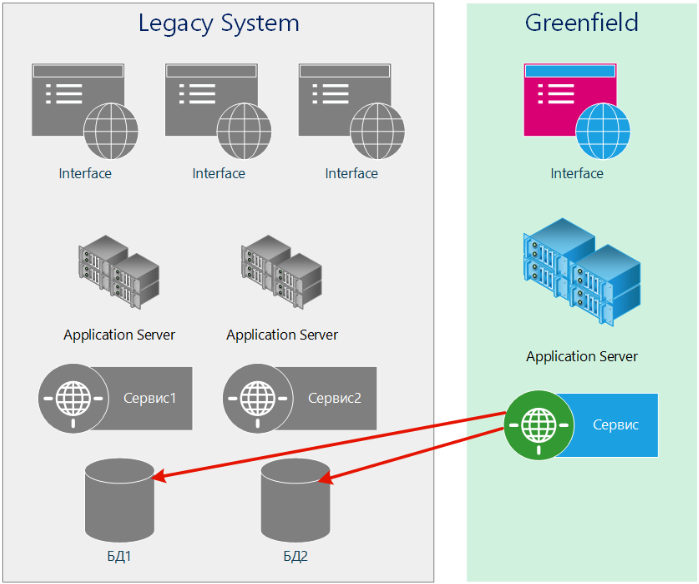
\includegraphics[width=0.6\textwidth]{stranglerApp.png}
\end{center}

\paragraph{Выделяйте (и переписывайте) отдельные модули.} Если создать новое <<приложение-душитель>> не получается, и код в текущем состоянии оставлять нельзя, то нам остается заняться постепенным рефакторингом и улучшением дизайна системы. Для этого релиз за релизом мы изолируем части системы, выделяем независимые модули и переписываем их. Таким образом, через определенное время большая часть системы будет переписана. Таким образом мы не устраиваем никаких революций, но скорость разработки может быть всё же ниже, так как переработка системы понемногу всё же происходит.

\subsection{Реинжиниринг}

Реинжиниринг~--- это повторная реализация унаследованной системы в целях повышения удобства ее эксплуатации и сопровождения. В это понятие входят разные процессы, среди которых документирование системы, её реорганизация и реструктуризация, перевод системы на один из более современных языков программирования, модификация и модернизация структуры и системных данных. При этом функциональность системы и, иногда, её архитектура остаются неизменными.

С технической точки зрения реинжиниринг~--- это решение <<второго сорта>> проблемы системной эволюции. Если учесть, что архитектура системы не изменяется, то сделать централизованную систему распределенной представляется делом довольно сложным. Также таким способом нельзя изменить язык программирования старых систем на современные языки (например, Go, F\# или Kotlin). Поэтому часто архитектуру тоже приходится менять, причём довольно радикально.

Однако с коммерческой точки зрения реинжиниринг часто принимается за единственный способ сохранения наследуемых систем в эксплуатации. Другие подходы к эволюции системы либо слишком дорогостоящие, либо рискованные. Чтобы понять причины такой позиции, следует рассмотреть проблемы, связанные с наследуемыми системами.

Код эксплуатируемых в настоящее время программных систем чрезвычайно огромен. В 1990 году насчитали порядка 120 млрд. строк исходного кода эксплуатируемых в то время программ. При этом большинство программ были написаны на языке COBOL, который лучше всего подходит для обработки данных в деловой сфере, и на языке FORTRAN. У этих языков достаточно ограниченные возможности в плане структуризации программ, a FORTRAN к тому же отличается ограниченной поддержкой структурирования данных. Несмотря на постоянную замену подобных систем, многие из них все еще используются. С 1990 года отмечается резкое возрастание использования вычислительной техники в деловой сфере. При грубом подсчете можно говорить о 250 млрд. строк исходного кода, которые нуждаются в сопровождении. Большинство создано отнюдь не с помощью объектно-ориентированных языков программирования, многие из них функционируют все еще на мэйнфреймах.

Программных систем настолько много, что говорить о полной замене или радикальной реструктуризации их в большинстве организаций не приходится. Сопровождение старых систем действительно стоит дорого, однако реинжиниринг может продлить время их существования. Как отмечалось ранее, реинжиниринг систем выгоден в том случае, если система обладает определенной коммерческой ценностью, но дорога в сопровождении. С помощью реинжиниринга совершенствуется системная структура, создается новая документация и облегчается сопровождение системы.

По сравнению с более радикальными подходами к совершенствованию систем реинжиниринг имеет два преимущества.

\begin{enumerate}
    \item Снижение рисков. При повторной разработке программного обеспечения существуют большие риски: высока вероятность ошибок в системной спецификации и возникновения проблем во время разработки системы. Реинжиниринг снижает эти риски.
    \item Снижение затрат. Себестоимость реинжиниринга значительно ниже, чем разработка нового программного обеспечения. В одной статье 1990 года приводится пример системы, эксплуатируемой в коммерческой структуре, повторная разработка которой оценивалась в 50 млн. долларов. Для этой системы был успешно выполнен реинжиниринг стоимостью всего 12 млн. долларов. Приведенные цифры типичны: считается, что реинжиниринг в четыре раза дешевле, чем повторная разработка системы.
\end{enumerate}

Реинжиниринг программного обеспечения тесно связан с реинжинирингом бизнес-процессов. Последний означает преобразование бизнес-процессов для снижения количества излишних видов деятельности и повышения эффективности делового процесса. Обычно реинжиниринг бизнес-процессов предполагает внедрение новых программ для поддержки деловых процессов или модификацию существующих программ, при этом наследуемые системы существенно зависят от делового процесса. Такую зависимость следует выявлять как можно раньше и устранять, прежде чем начнется планирование каких-либо изменений в самом бизнес-процессе. Поэтому решение о реинжиниринге программного обеспечения может возникнуть, если наследуемую систему не удается адаптировать к новым деловым процессам путем изменений в обычном сопровождении системы.

Основное различие между реинжинирингом и новой разработкой системы связано со стартовой точкой начала работы над системой. При реинжиниринге вместо написания системной спецификации <<с нуля>> старая система служит основой для разработки спецификации новой системы. В сравнении с реинжинирингом традиционная разработка программного обеспечения часто называется <<разработкой вперед>> (forward engineering). Традиционная разработка начинается с этапа создания системной спецификации, за которой следует проектирование и реализация новой системы. Реинжиниринг основывается на существующей системе, которая разработчиками изучается и преобразуется в новую.

\begin{center}
    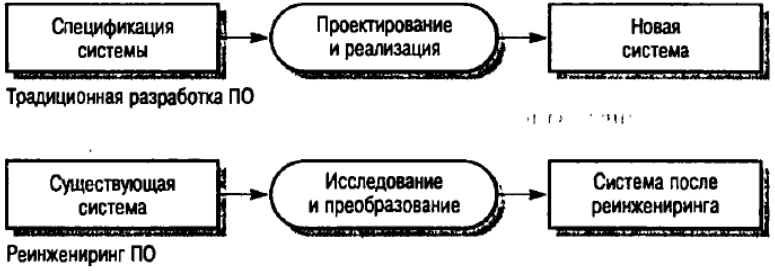
\includegraphics[width=0.7\textwidth]{developmentVsReengineering.png}
\end{center}

Стоимость реинжиниринга обычно определяется объемом выполненных работ. На рисунке ниже показано несколько различных подходов к процессу реинжиниринга и динамика изменения стоимости работ для этих подходов.

\begin{center}
    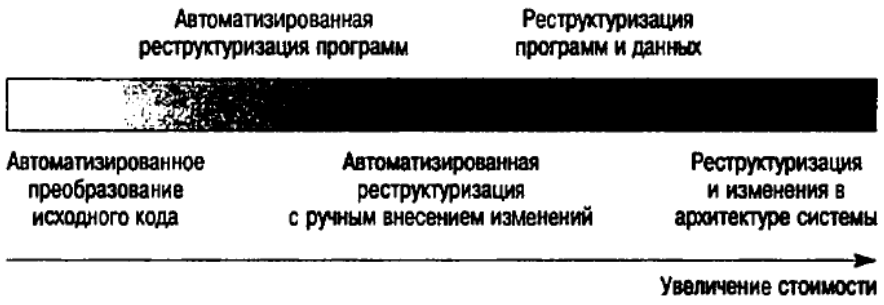
\includegraphics[width=0.7\textwidth]{reengineeringAutomation.png}
\end{center}

Кроме объема выполняемых работ, есть и другие факторы, обусловливающие стоимость реинжиниринга.

\begin{itemize}
    \item \textbf{Качество программного обеспечения, которое подвергается реинжинирингу}. Чем ниже качество программ и их документации (если она есть в наличии), тем выше стоимость реинжиниринга.
    \item \textbf{Наличие средств поддержки процесса реинжиниринга}. Обычно реинжиниринг экономически выгоден, если применяются средства для автоматизированного внесения изменений в программы.
    \item \textbf{Объем необходимого преобразования данных}. Стоимость процесса реинжиниринга возрастает при увеличении объема преобразуемых данных.
    \item \textbf{Наличие необходимых специалистов}. Если персонал, который занимается сопровождением системы, не может выполнить реинжиниринг, это также может стать причиной повышения стоимости процесса. Вновь привлеченные специалисты потратят много времени на изучение системы.
\end{itemize}

Основным недостатком реинжиниринга принято считать то, что с его помощью систему можно улучшить только до определенной степени. Основные архитектурные изменения или полную реструктуризацию программ невозможно выполнить автоматически, что также увеличивает стоимость реинжиниринга. И, несмотря на то, что реинжиниринг поможет улучшить сопровождение системы, все равно она будет намного хуже в сопровождении, чем новая, созданная с помощью современных методов инженерии программного обеспечения.

\subsubsection{Процесс реинжиниринга}

На следующем рисунке показан возможный процесс реинжиниринга. В начале этого процесса имеем наследуемую систему, а в результате~--- структурированную и заново скомпонованную версию той же системы. 

\begin{center}
    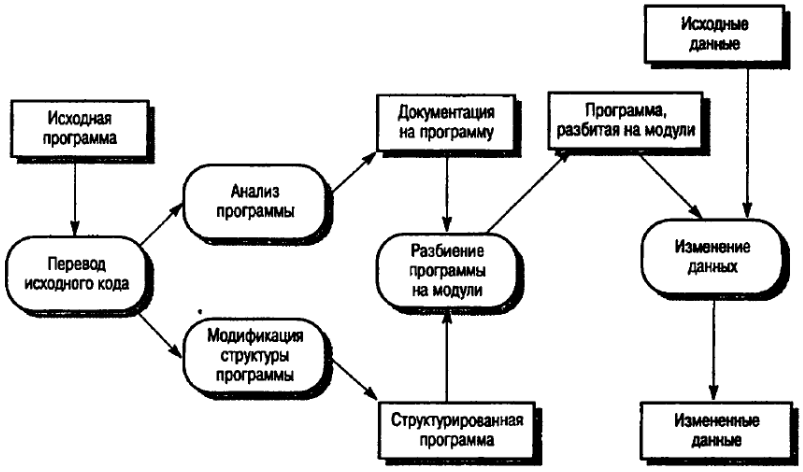
\includegraphics[width=0.8\textwidth]{reengineeringProcess.png}
\end{center}

При каждом конкретном реинжиниринге программ необязательно проходить все стадии, показанные на рисунке. Например, не всегда нужно переводить исходный код, если язык программирования, на котором написана программа, всё ещё всех устраивает и не будет меняться. Если реинжиниринг проводится с помощью автоматизированных средств, то не обязательно восстанавливать документацию на программу. Изменение системных данных необходимо, если в результате реинжиниринга изменяется их структура. Однако реструктуризация данных в процессе реинжиниринга требуется всегда.

Обсудим основные этапы этого процесса.

\paragraph{Перевод исходного кода}~--- конвертирование программы со старого языка программирования на современную версию того же языка либо на другой язык. Преобразование исходного кода будет эффективным только тогда, когда есть возможность выполнить основной перевод автоматически. Это может сделать либо специально созданная программа, либо коммерческая программа по конвертированию кода с одного языка в другой, либо система, основанная на поиске по шаблонам. В последнем случае нужно создать список команд для описания перевода с одного языкового представления на другое. Параметризированные образцы исходного языка подвергаются сравнению и сопоставлению с такими же образцами в новом языке.

В некоторых случаях автоматизированный перевод становится невозможным. Например, если структурные компоненты исходного кода не имеют соответствия в новом языке или производится перевод между языками разных парадигм (например, с C на Haskell). В такой ситуации придется настраивать и совершенствовать создаваемую систему вручную.

\begin{center}
    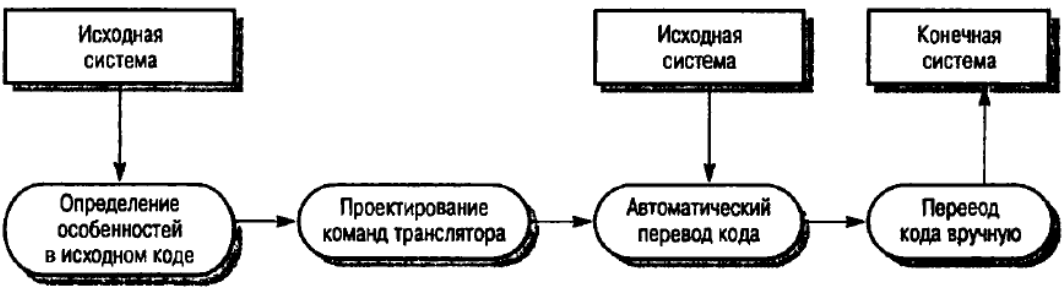
\includegraphics[width=0.8\textwidth]{sourceCodeTranslation.png}
\end{center}

\paragraph{Анализ программ.} Целью анализа является определение архитектуры и спецификации системы на основе ее исходного кода. Этот процесс не подразумевает изменения программ. Входными данными процесса анализа обычно служит исходный код системы. Однако зачастую даже он недоступен, тогда процесс анализа начинается с исполняемой программы. 

Вначале с помощью автоматизированных средств проводится анализ структуры системы. В большинстве случаев этого недостаточно для воссоздания системной архитектуры. Требуется дополнительная работа с исходным кодом системы и с моделью ее структуры. Эта дополнительная информация сравнивается с данными, собранными во время автоматического анализа системы, и представляется в виде ориентированного графа, отображающего связи в исходном коде программ.

\begin{center}
    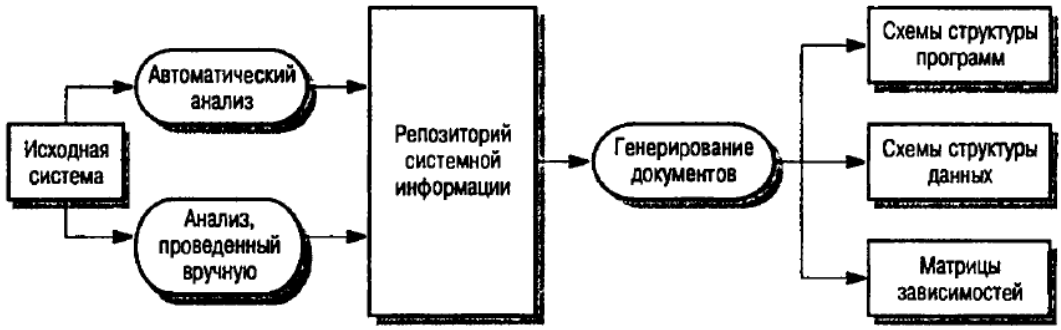
\includegraphics[width=0.8\textwidth]{programStructureAnalysis.png}
\end{center}

Репозиторий системной информации служит для сравнения структуры графа и кода. На основе данного графа можно получить такие документы, как схемы структуры программ и данных, а также матрицы зависимостей. Матрицы зависимостей показывают места определения в программах системных объектов и ссылки на них. Процесс разработки документации итеративный, так как информация о системной структуре используется для дальнейшего уточнения информации, которая хранится в системном репозитории.

После создания документации по системной архитектуре в репозитории вводится дополнительная информация, позволяющая восстановить системную спецификацию. Также зачастую составляют ручное описание структуры системы. 

\paragraph{Модификация структуры программ.} Если в процессе эксплуатации наследуемой системы возникла необходимость оптимизировать использование памяти и имеются проблемы с пониманием того, как она работает, это означает, что система плохо структурирована. Внутренняя структура legacy-систем часто значительно усложнена множеством безусловных переходов и нечеткой логикой программного кода. Регулярное сопровождение системы также не способствует сохранению системной структуры. После частых изменений некоторые фрагменты кода становятся неиспользуемыми, однако это можно обнаружить только после тщательного анализа программы.

\begin{center}
    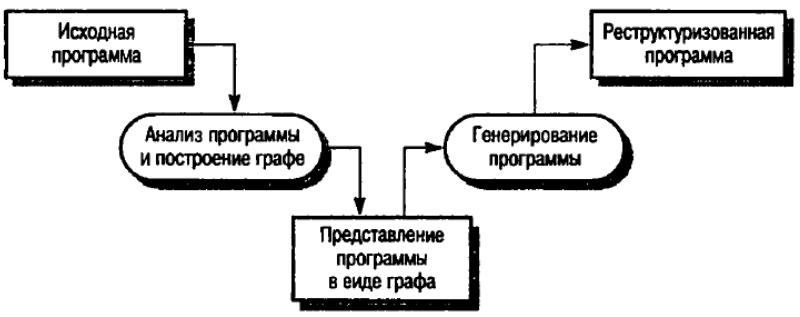
\includegraphics[width=0.7\textwidth]{programStructureReengineering.png}
\end{center}

Сначала программа представляется в виде ориентированного графа (графа потока управления), после чего создается структурированная программа без использования операторов перехода. К этому графу применяются методы упрощения и преобразования, в результате чего находятся и устраняются неиспользуемые части кода. После этого генерируется новая программа, при этом операторы безусловного перехода заменяются циклами и условными операторами. Такая программа может быть написана как на исходном языке, так и на любом другом (например, программу на языке FORTRAN можно сконвертировать в программу на С).

Автоматизированный способ реструктуризации программ имеет свои проблемы.

\begin{itemize}
    \item \textbf{Потеря комментариев}. Если в программе есть встроенные комментарии, они будут, скорее всего, утеряны в процессе реструктуризации.
    \item \textbf{Утрата связи с документацией}. По той же причине обычно нарушается соответствие между новой программой и документацией на исходную программу. Однако в большинстве случаев это не так уж важно, поскольку документация и комментарии уже устарели.
    \item \textbf{Жесткие требования к компьютерной технике}. Алгоритмы, встроенные в средства реструктуризации, отличаются высокой сложностью. При неаккуратной реализации процесс реструктуризации больших программ может занимать много времени.
\end{itemize}

Если программа находится под управлением данных и программные компоненты тесно связаны с используемыми структурами данных, реструктуризация кода не обязательно значительно улучшит программу. Если программа была написана с помощью редкого варианта языка программирования, стандартные средства преобразования структуры могут выполняться некорректно, поэтому неизбежно ручное вмешательство.

Иногда не стоит реструктуризировать все программы системы. Некоторые программы могут отличаться хорошим качеством, другие не подвергались большому количеству изменений, которые повредили бы их структуру. Для того, чтобы определить, какие компоненты системы следует подвергать реструктуризации в первую очередь, можно использовать следующие показатели:

\begin{itemize}
    \item интенсивность сбоев в работе программы;
    \item процентное соотношение кода, измененного на протяжении года;
    \item сложность компонент и другие метрики.
\end{itemize}

\paragraph{Разбиение на модули}~--- это процесс реорганизации программы в целях объединения ее взаимосвязанных частей в отдельном модуле. После этого легче удалить избыточность в соответствующих компонентах, оптимизировать взаимосвязи и упростить интерфейс всей программы. Например, в программе по обработке сейсмографических данных все операции по графическому представлению этих данных можно собрать в один модуль. Если система будет распределенной, модули можно инкапсулировать как объекты, доступ к которым будет осуществляться через общий интерфейс.

В программной системе можно выделить различные типы модулей.

\begin{enumerate}
    \item \textbf{Абстракции данных}. Это абстрактные типы данных, которые создаются путем объединения данных с компонентами их обработки. 
    \item \textbf{Аппаратные модули}. Тесно связаны с абстракцией данных и объединяют все функции, управляющие отдельными аппаратными устройствами.
    \item \textbf{Функциональные модули}. Объединяют все функции, которые выполняют сходные или взаимосвязанные задачи. Например, в один модуль можно объединить все функции, выполняющие ввод данных и их проверку. Этот подход применяется там, где создание абстракций данных невыгодно.
    \item \textbf{Модули поддержки отдельных процессов}. В них сгруппированы все функции и данные, отвечающие за поддержку отдельного бизнес-процесса. Например, в библиотечной системе присутствует модуль, объединяющий все функции, отвечающие за выдачу и возврат книг.
\end{enumerate}

Разбиение программы на модули обычно выполняется вручную путем проверки и правки кода. Для этого следует, прежде всего, определить взаимосвязи между компонентами и изучить способ их взаимодействия. Полностью автоматизировать этот процесс нельзя, даже если привлечь средства просмотра и визуализации программ.

\paragraph{Изменение системных данных.} До сих пор все обсуждаемые изменения касались в основном программ и систем. Однако в некоторых случаях придется столкнуться с проблемой изменения данных. Хранение, структура и формат данных, с которыми работает наследуемая система, должны измениться, чтобы соответствовать изменениям в программном обеспечении. Изменение данных~--- это процесс анализа и реорганизации структуры данных, а иногда еще и изменение значений системных данных.

В принципе, если функциональность системы осталась прежней, изменения данных не требуется. Однако существует ряд причин, которые вынуждают изменять данные (так же, как и программы) наследуемой системы.

\begin{itemize}
    \item \textbf{Нарушение данных}. С течением времени качество данных снижается. Изменения данных становятся причиной новых ошибок, возможно дублирование значений, изменения во внешнем окружении системы могут не найти адекватного отражения в данных. Эти явления неизбежны, так как время существования данных бывает достаточно большим. Например, персональные данные в банковской системе появляются с созданием нового счета и существуют, по меньшей мере, в течение всей жизни клиента. При изменении обстоятельств у клиента банковские данные должны обновляться, что не всегда происходит корректно. Реинжиниринг системы уменьшает эти трудности, что лишний раз подтверждает его необходимость.
    \item \textbf{Программные ограничения}. При разработке систем многие программисты включают в программы ограничения на количество обрабатываемых данных. Но согласно современным требованиям программы должны обрабатывать значительно больше данных, чем было предусмотрено изначально. Именно для устранения подобных ограничений может понадобиться изменение данных. В одной из книг, посвящённых реинжинирингу, приведен пример системы управления ценными бумагами, которая была способна обрабатывать до 99 транзакций за одну операцию. В компании, где эта система использовалась, осуществлялось управление 2000 транзакций, что вызвало необходимость в создании 23 копий системы. По этой причине впоследствии компания приняла решение о реинжиниринге системы и изменении данных.
    \item \textbf{Эволюция системной архитектуры}. При переходе от централизованной системы на распределенную ядром архитектуры должна стать система управления данными с удаленным доступом. Для перемещения данных из отдельных файлов на сервер СУБД может потребоваться большая работа по изменению этих данных.
\end{itemize}

Перед изменением данных необходимо провести подробный анализ программ, которые работают с этими данными. Главная цель анализа~--- определение в программе деклараций функций, выявление литеральных величин, требующих замены на именованные константы, поиск встроенных правил проверки данных. При анализе помогают такие средства, как анализаторы перекрестных ссылок и сопоставление с образцом. Для фиксации мест ссылок на элементы данных и изменений, которые там требуются, удобно создать набор таблиц регистрации изменений, которые содержат описание всех этапов изменения данных. Схема процесса изменения данных показана на следующем рисунке.

\begin{center}
    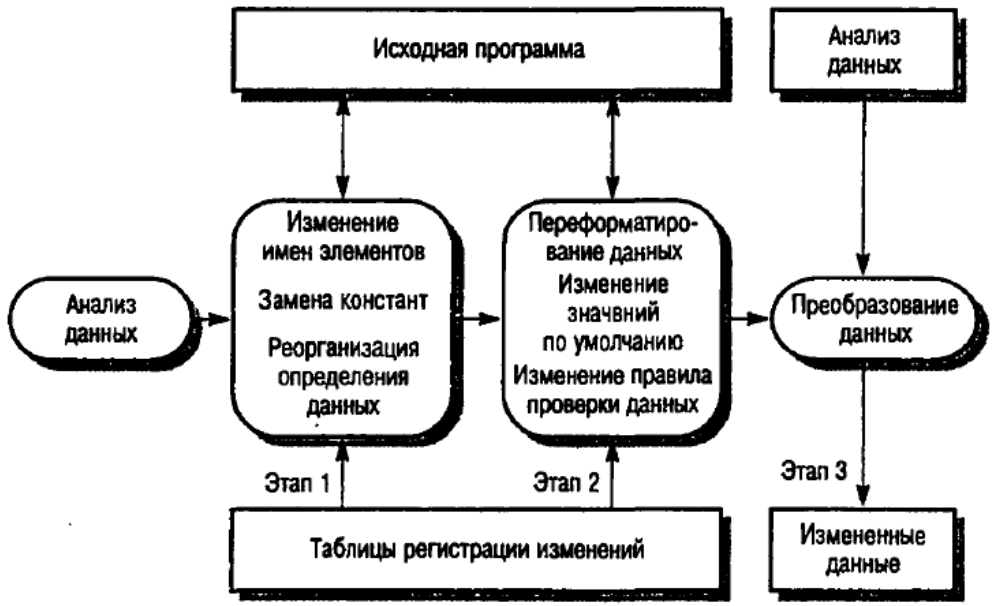
\includegraphics[width=0.75\textwidth]{dataReengineering.png}
\end{center}

На первом этапе процесса изменения данных модифицируются определения данных. На сами данные такая модификация не оказывает влияния. Чтобы автоматизировать этот процесс, можно использовать системы сопоставления с образцом, например awk, которые помогают находить и заменять определения, или же можно, например, создать XML-определения данных и использовать их для управления средствами конвертирования данных. Несмотря на это, ручной работы над данными практически невозможно избежать. Если ставится цель улучшить понимаемость определений данных, то работу можно остановить на этой стадии. Если же имеются проблемы со значениями данных, описанные выше, следует начать второй этап процесса изменения данных.

После второго этапа обязательно идет третий~--- преобразование данных. Обычно это очень дорогостоящий процесс. Для его реализации создаются программы, аккумулирующие информацию о старой и новой структурах данных. Здесь часто опять применяется система сопоставления с образцом.

\end{document}